\subsection{Auswertung der Zufriedenheit (H$_{3}$)}
\label{ch:Ergebnisse:sec:Hypothesen_Auswertung:sub:Zufriedenheit}
% Usability = 
% - Satisfaction: Do users find the system enjoyable and pleasant to use? Are they satisfied with the overall experience?
% Einfluss von Erwartungskonformität, Benutzerbindung, Steuerbarkeit

Nutzer sind mit einem System zufrieden, wenn sie die Nutzung angenehm und erfreulich finden. Dafür muss es den Erwartungen der Nutzer entsprechen, leicht steuer- und navigierbar sein und eine Bindung zum Nutzer aufbauen. Die Zufriedenheit lässt sich dabei nicht in metrischen Kenngrößen erfassen, stattdessen aber beispielsweise in Form eines Spektrums anhand von Fragebögen (s. \autoref{ch:SdF:UI:ISO}).
Folgende Hypothese ist zu bestätigen:
\begin{quote}
    H$_{3}$ = Die Nutzung des neuen Systems ($\mu2$) beeinflusst die Bewertung ($b$) der Software positiv im Vergleich zur Nutzung des alten Systems ($\mu1$); \\$b(\mu1) < b(\mu2)$.
\end{quote}

\noindent
\noindent
Auf Grundlage der jahrezehntelangen Erfahrung mit dem alten System ist anhand der Befragung festzustellen, dass manche der Nutzer einer Modernisierung ihrer Routine teilweise sehr kritisch gegenüber stehen. Auch wenn das neue System anhand der Bewertung aus dem vorherigen Kapitel sehr intuitiv ist, folgt daraus nicht unbedingt, dass der Nutzer es gut findet. Das Spektrum der Antworten der Nutzerumfrage sind in \autoref{fig:pruemper_all} in Form eines Box-Plot zusammengefasst. Trotz einzelner Ausreißer ist eine klare Tendenz erkennbar, dass das neue System besser bewertet wurde.

Diese grafische Tendenz bestätigt sich durch die Differenzen der Mittelwerte (s. \autoref{tab:Nutzerbefragung:Differenz+ttest}). Das Ergebnis des alten Systems wurde von dem des neues Systems abgezogen. Da die Differenz bei jeder Frage positiv ausfällt, wurde das neue System insgesamt besser bewertet als das alte.
 

\begin{figure}[H]
    \centering
    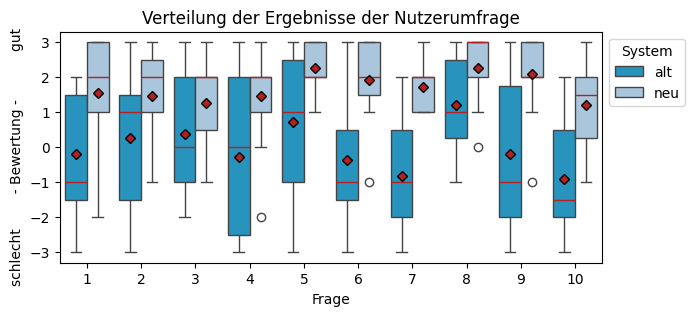
\includegraphics[width=1\linewidth]{Diagramme/pruemper_all.png}
    \caption{Auswertung der Nutzerbefragung (Daten aus \autoref{tab:Nutzerbefragung:rohe_Daten})}
    \label{fig:pruemper_all}
\end{figure}

\begin{table}[h]
\begin{center}
\begin{tabular}{|l|c|c|c|c|c|}
\hline
Frage                                   & 1      & 2      & 3      & 4      & 5      \\ \hline
$\varnothing_{neu} - \varnothing_{alt}$ & 1,73   & 1,18   & 0,91   & 1,73   & 1,55   \\ \hline
t-Test                                  & 0,0195 & 0,0949 & 0,1387 & 0,0487 & 0,0231 \\ \hline
\hline
Frage                                   & 6      & 7      & 8      & 9      & 10     \\ \hline
$\varnothing_{neu} - \varnothing_{alt}$ & 2,27   & 2,55   & 1,07   & 2,29   & 2,1   \\ \hline
t-Test                                  & 0,0087 & 0,0021 & 0,0286 & 0,021 & 0,02 \\ \hline
\hline
t-Test über alle $\varnothing$ & \multicolumn{5}{c|}{0,00000218748} \\ \hline
\end{tabular}
\caption{Nutzerbefragung - Differenz der Antwortmittelwerte und t-Test-Ergebnisse (Weiterverarbeitung der Daten aus \autoref{tab:Nutzerbefragung:rohe_Daten})}
\label{tab:Nutzerbefragung:Differenz+ttest}
\end{center}
\end{table}

\noindent
Weiterhin weisen 80\% der Fragen anhand der t-Test-Ergebnisse (s. \autoref{fig:Nutzerbefragung:ttest+Signifikanzniveau}) sowie das Ergebnis des t-Tests über alle durchschnittlichen Werte (s. \autoref{tab:Nutzerbefragung:Differenz+ttest}) einen statistisch signifikanten Unterschied auf.

\begin{figure}[H]
    \centering
    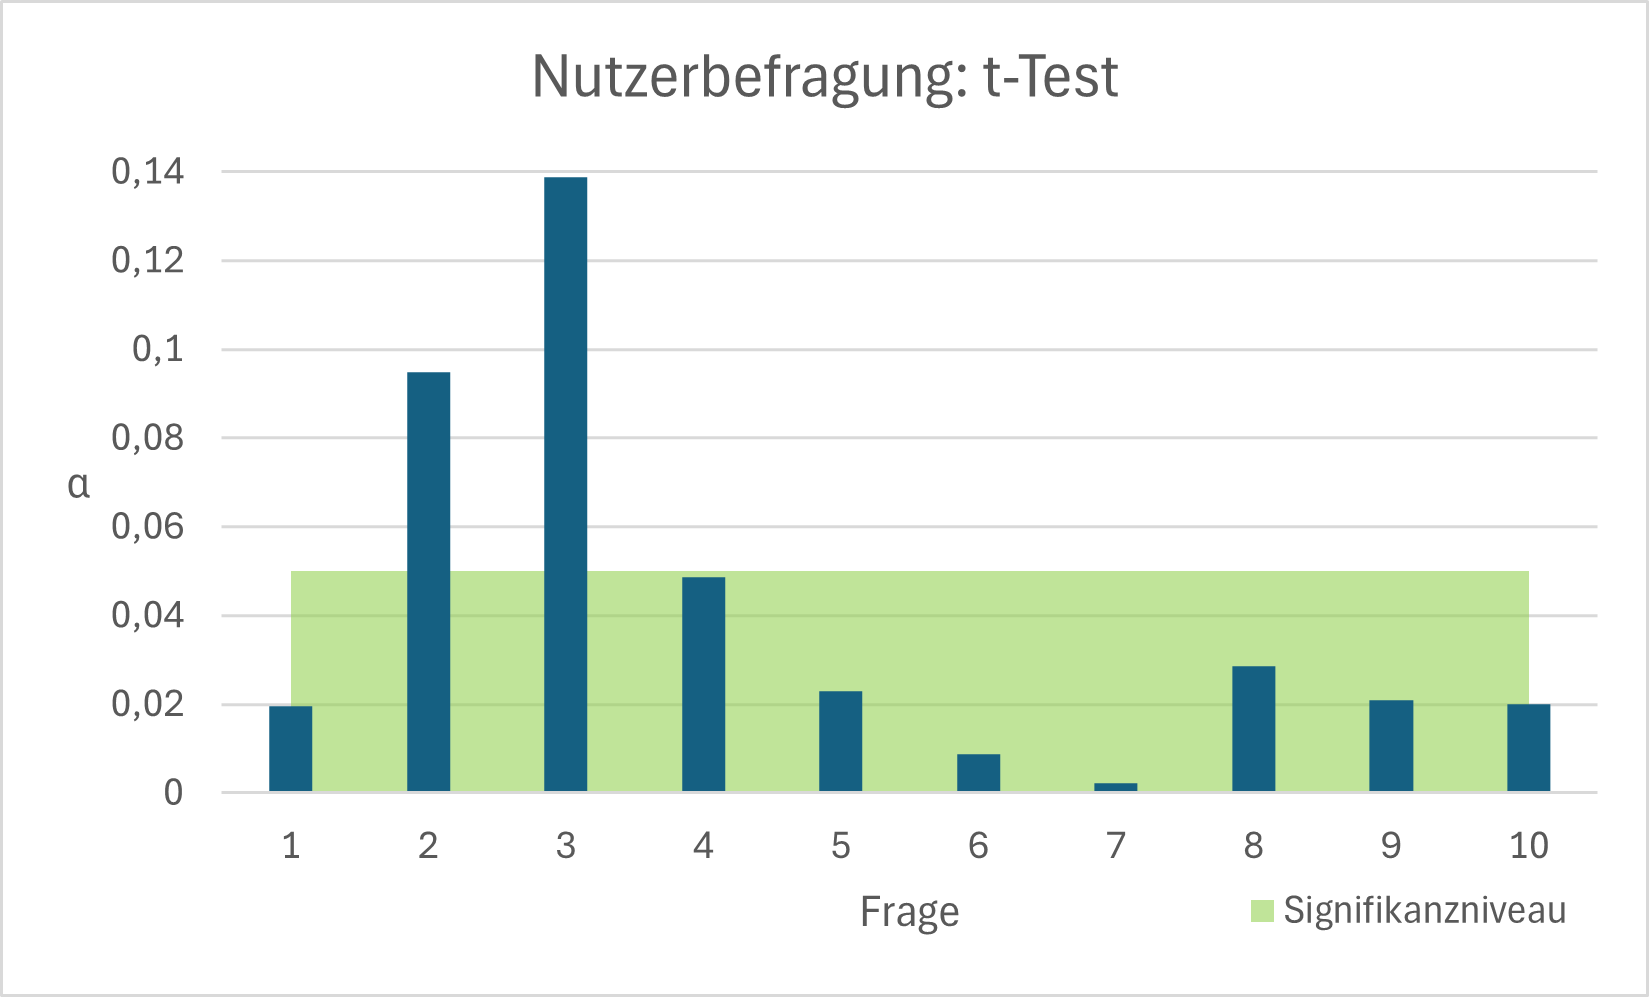
\includegraphics[width=0.8\linewidth]{Diagramme/pruemper_ttest.png}
    \caption{Signifikanzbewertung der Ergebnisse der Nutzerbefragung (Daten aus \autoref{tab:Nutzerbefragung:Differenz+ttest})}
    \label{fig:Nutzerbefragung:ttest+Signifikanzniveau}
\end{figure}

% *******************************************************************
%\subsection*{ISO-Kriterium Erwartungskonformität}

\begin{figure}[H]
    \centering
    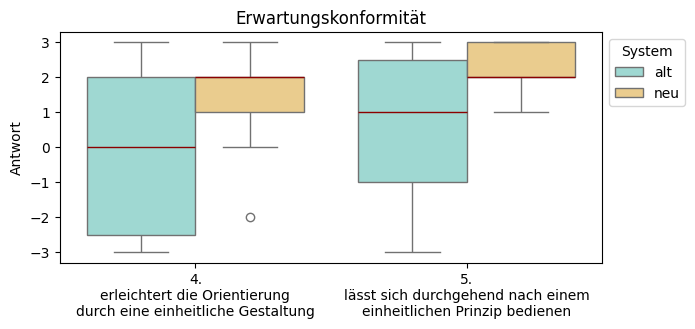
\includegraphics[width=1\linewidth]{Diagramme/pruemper_ek.png}
    \caption{Auswertung der Fragen bzgl. Gestaltungskriterium Erwartungskonformität nach ISO 9241-110 (Ausschnitt aus \autoref{fig:pruemper_all})}
    \label{fig:pruemper_Erwartungskonformität}
\end{figure}

\noindent
t-Test von Fragen 1 \& 8 sind signifikant (<0.5)\\
Boxplot: %\autoref{fig:pruemper_Erwartungskonformität}

%\subsection{ISO-Kriterium Benutzerbindung}
-> Abgrenzung von UX(!)
%\subsection*{Einfluss von ISO-Steuerbarkeit}
%\autoref{fig:pruemper_Steuerbarkeit}
%\subsection*{weitere: Erlernbarkeit}

\noindent
Die ISO-Prinzipien, die sich spezieller auf das Kriterium der Zufriedenheit beziehen, sind die Erwartungskonformität (s. \autoref{fig:pruemper_Erwartungskonformität}), die Steuerbarkeit (s. \autoref{fig:pruemper_Steuerbarkeit}) und die Benutzerbindung, welche nicht durch den Fragebogen repräsentiert wurde (s. \autoref{Add:Nutzerbefragung_Prümper:Begründung_Filterung}).

Allgemein sind die Nutzer sehr zufrieden mit dem neuen Dash\-board. 80\% der Fragen haben ein signifikant besseres Ergebnis bezüglich des Dash\-boards erhalten. Nach Ausfilterung der zwei bereits genannten Ausnahmen (s. \autoref{ch:Ergebnisse:sec:Hypothesen_Auswertung:sub:Effektivität}), welche zudem die mit Abstand größte Expertise aufweisen (s. \autoref{Add:Mitschriften_Mitarbeiteraussagen}), steigt dieser Wert auf 100\%.

Auf Grundlage der vorliegenden Ergebnisse hat das Dashboard einen signifikant positiven Einfluss auf den Monitoring"=Prozess. Somit kann die Hypothese $H_{13}$ akzeptiert werden.

\begin{figure}[H]
    \centering
    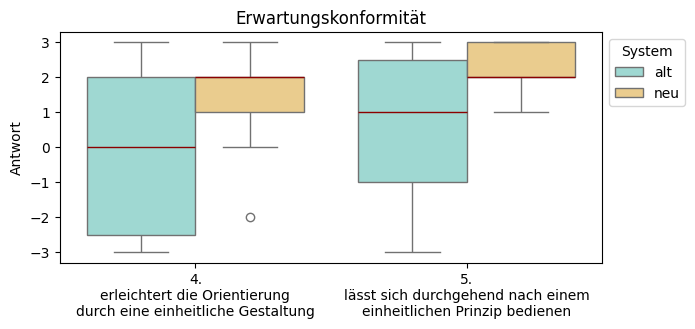
\includegraphics[width=1\linewidth]{Diagramme/pruemper_ek.png}
    \caption{Auswertung der Fragen bzgl. Gestaltungskriterium Erwartungskonformität nach ISO 9241-110 (Ausschnitt aus \autoref{fig:pruemper_all}) \textcolor{red}{TODO: Titel}}
    \label{fig:pruemper_Erwartungskonformität}
\end{figure}

% ******************************************************************
%           Subjektive Daten - Begründung Zufriedenheit
% ******************************************************************
% Allgemein
%Nutzer sind zufrieden damit\\
%--> Es lässt sich zusammenfassend sagen, dass die Nutzer sehr zufrieden mit dem neuen Dashboard sind.\\
%--> Prümper\\
%--> Gibt es eine Diskrepanz zwischen Nutzen und Nutzbarkeit eines System (obj / subj)?\\
%\textbf{Decken sich die Ergebnisse der Umfrage und des Tests?}\\
%-	wie sich gemessene Werte und Umfrageergebnisse decken / bestätigen\\
%-	Bewerten in jeder Nuance\\
%  --> moderierende Variablen, Effizienz/Zeit, Effektivität/Genauigkeit, Umfrage\\
%  --> alles in die Kategorien der ISO-Norm???\\


% ****************************************************************
\noindent
Zusätzlich zu der detaillierten Bewertung der Systeme wurde auch abgefragt, für wie wahrscheinlich es die Teilnehmer halten, das Dash\-board in Zukunft zu nutzen (s. \autoref{fig:DB_Nutzung:boxplot}). Da im Vergleich zu den anderen t-Tests nur eine Datenreihe vorliegt, wurde das Ergebnis mit Null paarweise, einseitig verglichen, also mit der neutralen Einstellung gegenüber beider Systeme. Bis auf die selben zwei Personen, die ein klares 'nein' antworteten, haben alle weiteren Testpersonen mit 'eher ja' und 'ja' geantwortet. Auch der t-Test bestätigt eine statistische Signifikanz dieser Aussage. Dieses Ergebnis ist daher mit einem positiven Durchschnitt statistsich signifikant.

Ausgehend von diesem Ergebnis kann auch die Hypothese $H_{13}$ akzeptiert werden.

\begin{table}[H]
    \centering
    \begin{tabular}{|c|c|c|c|c|c|c|c|c|c|c||c|c|c|}
        \hline
        \multicolumn{11}{|l||}{Antworten der Nutzer} & $\varnothing$ & $\Bar{x} $ & t-Test \\ \hline
        -2 & 2 & 1 & 2 & 2 & 1 & 2 & 2 & 2 & 1 & -2 & 1 & 2 & 0,028974853 \\ \hline
    \end{tabular}
    \caption{Ergebnisse der Umfrage zur Wahrscheinlichkeit der eigenen zukünftigen Dash\-board"=Nutzung (Daten aus \autoref{tab:Nutzerbefragung:rohe_Daten})}
    \label{tab:DB_Nutzung:rohe_Daten}
\end{table}

\begin{figure}[H]
    \centering
    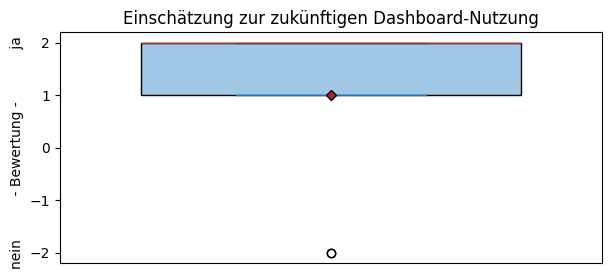
\includegraphics[width=1\linewidth]{Diagramme/dashboard_use.png}
    \caption{Antwortverteilung %der Frage 
    bzgl. der Wahrscheinlichkeit zur zukünftigen Dashboard"=Nutzung (Daten aus \autoref{tab:DB_Nutzung:rohe_Daten})}
    \label{fig:DB_Nutzung:boxplot}
\end{figure}
